%%%%%%%% ICML 2026 EXAMPLE LATEX SUBMISSION FILE %%%%%%%%%%%%%%%%%

\documentclass{article}

% Recommended, but optional, packages for figures and better typesetting:
\usepackage{microtype}
\usepackage{graphicx}
\usepackage{subcaption}
\usepackage{booktabs} % for professional tables

% hyperref makes hyperlinks in the resulting PDF.
% If your build breaks (sometimes temporarily if a hyperlink spans a page)
% please comment out the following usepackage line and replace
% \usepackage{icml2026} with \usepackage[nohyperref]{icml2026} above.
\usepackage{hyperref}


% Attempt to make hyperref and algorithmic work together better:
\newcommand{\theHalgorithm}{\arabic{algorithm}}
% Use the following line for the initial blind version submitted for review:
\usepackage{icml2026}

% For preprint, use
% \usepackage[preprint]{icml2026}

% If accepted, instead use the following line for the camera-ready submission:
% \usepackage[accepted]{icml2026}

\usepackage{amsmath}
\usepackage{amssymb}
\usepackage{mathtools}
\usepackage{amsthm}


% if you use cleveref..
\usepackage[capitalize,noabbrev]{cleveref}

%%%%%%%%%%%%%%%%%%%%%%%%%%%%%%%%
% THEOREMS
%%%%%%%%%%%%%%%%%%%%%%%%%%%%%%%%
\theoremstyle{plain}
\newtheorem{theorem}{Theorem}[section]
\newtheorem{proposition}[theorem]{Proposition}
\newtheorem{lemma}[theorem]{Lemma}
\newtheorem{corollary}[theorem]{Corollary}
\theoremstyle{definition}
\newtheorem{definition}[theorem]{Definition}
\newtheorem{assumption}[theorem]{Assumption}
\theoremstyle{remark}
\newtheorem{remark}[theorem]{Remark}

% Todonotes is useful during development; simply uncomment the next line
%    and comment out the line below the next line to turn off comments
%\usepackage[disable,textsize=tiny]{todonotes}
\usepackage[textsize=tiny]{todonotes}

\usepackage{tikz}
\usetikzlibrary{positioning, fit, shapes}
\usetikzlibrary{shapes.geometric, arrows.meta, positioning, calc}

% Toggle
\newcommand{\showcomments}{1} % set to 0 to hide

% Generic comment
\newcommand{\authcomment}[3]{%
\ifnum\showcomments=1
  {\textcolor{#2}{\textbf{[#1: #3]}}}%
\fi}
\newcommand{\st}[1]{\authcomment{Sang}{blue}{#1}}
\newcommand{\md}[1]{\authcomment{Duc}{orange}{#1}}



% The \icmltitle you define below is probably too long as a header.
% Therefore, a short form for the running title is supplied here:
\icmltitlerunning{Reliable and Efficient Amortized Model-based Evaluation for AI Agents}

\begin{document}

\twocolumn[
  \icmltitle{Reliable and Efficient Amortized Model-based Evaluation for AI Agents}

  % It is OKAY to include author information, even for blind submissions: the
  % style file will automatically remove it for you unless you've provided
  % the [accepted] option to the icml2026 package.

  % List of affiliations: The first argument should be a (short) identifier you
  % will use later to specify author affiliations Academic affiliations
  % should list Department, University, City, Region, Country Industry
  % affiliations should list Company, City, Region, Country

  % You can specify symbols, otherwise they are numbered in order. Ideally, you
  % should not use this facility. Affiliations will be numbered in order of
  % appearance and this is the preferred way.
  \icmlsetsymbol{equal}{*}

  \begin{icmlauthorlist}
    \icmlauthor{Firstname1 Lastname1}{equal,yyy}
    \icmlauthor{Firstname2 Lastname2}{equal,yyy,comp}
    \icmlauthor{Firstname3 Lastname3}{comp}
    \icmlauthor{Firstname4 Lastname4}{sch}
    \icmlauthor{Firstname5 Lastname5}{yyy}
    \icmlauthor{Firstname6 Lastname6}{sch,yyy,comp}
    \icmlauthor{Firstname7 Lastname7}{comp}
    %\icmlauthor{}{sch}
    \icmlauthor{Firstname8 Lastname8}{sch}
    \icmlauthor{Firstname8 Lastname8}{yyy,comp}
    %\icmlauthor{}{sch}
    %\icmlauthor{}{sch}
  \end{icmlauthorlist}

  \icmlaffiliation{yyy}{Department of XXX, University of YYY, Location, Country}
  \icmlaffiliation{comp}{Company Name, Location, Country}
  \icmlaffiliation{sch}{School of ZZZ, Institute of WWW, Location, Country}

  \icmlcorrespondingauthor{Firstname1 Lastname1}{first1.last1@xxx.edu}
  \icmlcorrespondingauthor{Firstname2 Lastname2}{first2.last2@www.uk}

  % You may provide any keywords that you find helpful for describing your
  % paper; these are used to populate the "keywords" metadata in the PDF but
  % will not be shown in the document
  \icmlkeywords{Machine Learning, ICML}

  \vskip 0.3in
]

% this must go after the closing bracket ] following \twocolumn[ ...

% This command actually creates the footnote in the first column listing the
% affiliations and the copyright notice. The command takes one argument, which
% is text to display at the start of the footnote. The \icmlEqualContribution
% command is standard text for equal contribution. Remove it (just {}) if you
% do not need this facility.

% Use ONE of the following lines. DO NOT remove the command.
% If you have no special notice, KEEP empty braces:
\printAffiliationsAndNotice{}  % no special notice (required even if empty)
% Or, if applicable, use the standard equal contribution text:
% \printAffiliationsAndNotice{\icmlEqualContribution}

\begin{abstract}
Evaluating large language models agents on new benchmarks is expensive, requiring costly infrastructure and inference. A natural question is whether we can predict model performance on unseen items by decomposing existing evaluations into latent capability factors. We propose an amortized model-based evaluation method tailored to agentic evaluation, which leverages the rich semantic structure of benchmark tasks by learning a global projection from item embeddings to multidimensional factor loadings. This enables zero-shot prediction on new items without re-estimation. Our approach automatically discovers the effective dimensionality of capability space and leverages fine-grained feedback from agent execution traces to disentangle correlated factors. The validity of discovered factors depends on item quality: many benchmark items are ill-posed---requiring packages not permitted by the environment or referencing inaccessible information---causing agent failures that do not reflect true capability. Since such items distort the validity of discovered latent factors, we develop an automated item revision pipeline to identify and fix these defects. With valid items, the discovered latent factors become interpretable: Sparse Autoencoder analysis recovers meaningful capability axes such as statistical scripting, Python debugging, and agentic tool-use. Experiments on 10 agentic benchmarks and 40 LLMs show that this approach is more reliable and efficient compared to current common practice.
\end{abstract}

% \section{Introduction}
% Motivation for evaluation in latent dimension. The need for generalization. 

% Agentic system has diverse and multidimentional skills. Understanding their strength and weakness is important

% Contribution 1: We propose a latent variable that discover these skills through data
% Contribution 2: Interpreting the latent dimension via SAE
% Contribution 3: Automatic item reviser workflow 

\section{Introduction}
% maybe lead with predictive 
% generative model has more skills --> surge of interest to use the AI system in diverses. This is because genAI is believed to have generalizable applicability by composition the elementary skills that it has learn % https://arxiv.org/pdf/2409.19808

% Evaluation for generative systems often collect from the field, as oppose to specifically design to measure a particular skill. This has higher utility for the particular field/domain of evaluation, but it has limited generalizable insight cross domain

% generalization is important because evaluate a system on a new items in new domain is expensive (docker, cost of inference). it would be beneficial to accurately infer model performance on new items by decomposition exisiting performance into subskills. 

% existing methods for decomposition like HELM profiles or General Scale is incompleted because it relies on prior knowledge annotation, which make it less predictive. There is a desire to capture more variance for better predictive performance

% Latent variable model, such as factor model, offers a data-driven method to capture variance in the latent space of the model. Classific factor model, which has free parameters for each items and test takers, relies on large number of test takers to identify latent structure. We construct a probabilistic factor model with amortization and automatic rank selection via a bayesian prior. This probabilistic structure also allow us to leverage finegrained feedback from the evaluation. 

As generative models integrate increasingly diverse capabilities — from reasoning and coding to agentic planning - the evaluation has moved from a single aggregate scores to characterizing models via multi-dimensional scales that map performance across distinct axes of capability \cite{liang2022holistic, zhou2025general}. While this shift toward profiling is a crucial step forward, current approaches remain predominantly prescriptive, relying on pre-defined taxonomies—whether manually curated dataset tags (e.g., ``machine learning engineering'', ``competitive programming'') or rubrics for specific traits (e.g., ``instruction following'') \cite{zhou2025general}. These methods implicitly assume that the ontology of AI capabilities is known, static, and fully captured by the evaluator's definitions. This prescriptive approach is insufficient for the dynamic landscape of AI. The capabilities of AI systems are not static but emergent. Over time, the AI population evolves and unlock new capability.

To capture this open-ended evolution, evaluation must become \textbf{descriptive}. We need statistical methods that can \textit{discover} the latent profile of a model directly from its behavior, without relying on rigid, pre-specified categories.

Latent variable models, such as Factor Analysis and Item Response Theory (IRT), provide the classical mathematical foundation for this discovery \cite{spearman1904proof, lord1980applications}. By decomposing observed responses into latent abilities and item properties, these methods can empirically disentangle the "true" dimensions of variance driving performance. However, applying these classical methods to the GenAI ecosystem faces a unique statistical barrier: the \textbf{identifiability bottleneck}.

Classical psychometrics operates in a "large-sample" regime ($N \to \infty$), identifying latent factors via the consensus of thousands of test-takers. GenAI evaluation operates in an inverted regime: a small, fixed population of models ($N \approx 50$) is evaluated on a massive universe of benchmarks ($J \approx 10^5$). As we detail in Section \ref{sec:motivation}, this rank deficiency ($N \ll J$) renders standard data-driven profiling mathematically unidentifiable; there are simply more degrees of freedom than there are models to constrain them.

In this work, we propose an \textbf{Amortized Factor Model} that addresses this challenge to enable rigorous, data-driven profiling of GenAI models. We introduce three methodological innovations:

\begin{itemize}
    \item \textbf{Amortized Discovery:} We replace free item parameters with an amortized function of semantic content. By learning a global projection from item embeddings to factor loadings, we decouple the model's degrees of freedom from the benchmark size, enabling the discovery of high-dimensional capability profiles even when $N$ is small.
    \item \textbf{Adaptive Dimensionality (ARD):} We employ Automatic Relevance Determination to resolve the dynamic ontology problem. Rather than pre-specifying the number of profile axes, our model uses sparsity-inducing priors to automatically discover the effective dimensionality of the capability space, adapting as new benchmarks and skills emerge.
    \item \textbf{Fine-Grained Feedback:} We move beyond binary correctness by integrating granular signals (e.g., subskill traces) as auxiliary supervision, increasing the information density available to disentangle correlated latent factors.
\end{itemize}

We demonstrate that this approach recovers interpretable, data-driven profiles that not only correlate with human-defined taxonomies but also reveal hidden structures in model performance that manual rubrics miss.

\paragraph{Contributions.} In summary, our contributions are the following:
\begin{enumerate}
    \item \textbf{Amortized Factor Model.} We introduce an amortized factor model that enables efficient generalization to new evaluation items through learned projections from item embeddings to factor loadings, ARD-based automatic dimensionality discovery, and fine-grained subskill feedback. On 25 benchmarks spanning LLMs and AI agents, we achieve over 15\% AUC improvement compared to Rasch and naive baselines (Section~\ref{sec:experiments}).

    \item \textbf{Automated Benchmark Remediation.} We develop a Judge-Guided Dual-Repair pipeline that automatically identifies and fixes benchmark defects through environmental patches and item-level corrections, reducing false-positive defect rates from 44.6\% to 0\% (Section~\ref{sec:item_fixing}).

    \item \textbf{Interpretable Latent Factors via SAE Analysis.} We demonstrate that discovered latent dimensions can be interpreted through Sparse Autoencoder (SAE) feature analysis, recovering meaningful capability axes---such as R scripting, Python debugging, and agentic tool-use---that correlate with human-defined taxonomies while revealing hidden structure that manual rubrics miss (Section~\ref{sec:interpretation}).
\end{enumerate}

\section{Related Work}

Our work lies at the intersection of psychometric measurement theory, large language model evaluation, and mechanistic interpretability. We review relevant literature across these domains.

\paragraph{Item Response Theory and Psychometrics.}
The statistical foundations of latent trait measurement originate with Spearman's factor analysis \cite{spearman1904proof} and were formalized through Item Response Theory (IRT) \cite{lord1980applications, embretson2000item}. The Rasch model \cite{rasch1960probabilistic} posits a single latent ability dimension, while the two-parameter logistic (2PL) model \cite{birnbaum1968latent} adds item discrimination. Multidimensional IRT (MIRT) \cite{reckase2009multidimensional} extends these frameworks to vector-valued abilities, enabling richer profiling. However, all classical IRT approaches assume large test-taker populations ($N \to \infty$) for consistent estimation \cite{anderson1956statistical}---an assumption violated in AI evaluation where $N$ is small and fixed. Our amortization strategy addresses this by decoupling parameter count from sample size.

\paragraph{Automatic Relevance Determination and Sparse Priors.}
Bayesian approaches to automatic dimensionality selection have a rich history. MacKay's Automatic Relevance Determination (ARD) \cite{mackay1995probable} uses hierarchical priors to prune irrelevant input dimensions in neural networks. Neal \cite{neal1996bayesian} extended these ideas to full Bayesian neural network training. In the context of latent variable models, sparsity-inducing priors enable data-driven discovery of the effective latent dimensionality \cite{tipping1999probabilistic, blei2003latent}. Our use of Laplace priors with ReLU reparameterization follows this tradition, achieving exact sparsity (rather than soft shrinkage) to automatically determine the number of capability factors.

\paragraph{Amortized Inference.}
The principle of amortizing inference---learning a function that maps observations to posterior parameters rather than optimizing per-instance---was popularized by variational autoencoders \cite{kingma2014auto} and has cognitive science antecedents \cite{gershman2014amortized}. We apply amortization in a novel context: rather than amortizing over data instances, we amortize over \textit{items}, learning a global projection from item embeddings to factor loadings. This transforms the identifiability condition from $N \ge K$ to $N \ge Kd/(J-K)$, enabling high-dimensional latent spaces with small model populations.

\paragraph{LLM Evaluation and Benchmarking.}
The evaluation of large language models has evolved from single-metric leaderboards to multi-dimensional profiling. HELM \cite{liang2022holistic} introduced holistic evaluation across scenarios, metrics, and models. BIG-bench \cite{srivastava2022beyond} scaled to hundreds of tasks, while MMLU \cite{hendrycks2021measuring} focused on knowledge-intensive domains. For open-ended generation, LLM-as-a-Judge approaches \cite{zheng2023judging} and human preference platforms like Chatbot Arena \cite{chiang2024chatbot} employ Elo-style ratings \cite{elo1978rating}. Agent-specific benchmarks such as AgentBench \cite{liu2023agentbench} and frameworks like ReAct \cite{yao2023react} and Reflexion \cite{shinn2023reflexion} evaluate agentic capabilities. Our work complements these efforts by providing a principled statistical framework for discovering latent capability dimensions from evaluation data.

\paragraph{Benchmark Contamination and Gaming.}
As LLMs are trained on increasingly large web corpora, benchmark contamination---where test items appear in training data---has emerged as a critical concern \cite{sainz2023nlp, oren2024proving, zhou2023dont}. Models may exploit memorized answers rather than exhibiting genuine capability, inflating performance metrics \cite{jacovi2023stop}. While prior work focuses on detecting contamination, our robust estimation framework (Section~\ref{sec:contamination}) takes a complementary approach: using fine-grained feedback signals to identify and downweight contaminated responses, enabling consistent capability estimation even under strategic distortion.

\paragraph{Sparse Autoencoders for Interpretability.}
Recent advances in mechanistic interpretability have demonstrated that Sparse Autoencoders (SAEs) can decompose neural network activations into interpretable, monosemantic features \cite{bricken2023monosemanticity, cunningham2023sparse}. This builds on theoretical work showing that neural networks learn superposed representations \cite{elhage2022toy}. We apply SAE-based analysis in a novel direction: rather than interpreting model internals, we use SAEs to interpret the \textit{latent factors} discovered by our evaluation framework, recovering human-readable capability descriptions from otherwise opaque dimensions.

\paragraph{Emergent Capabilities and Scaling.}
The phenomenon of emergent capabilities---abilities that appear discontinuously as models scale \cite{wei2022emergent, kaplan2020scaling}---poses challenges for evaluation. Static benchmarks designed for current models may fail to discriminate future models, while entirely new capability dimensions may emerge. Our ARD-based approach addresses this by treating dimensionality as a data-driven property, allowing the capability space to grow or shrink as the model population and benchmark suite evolve.

\section{Method}
\subsection{Probabilistic Model}
We propose a probabilistic model integrating amortized item representations with Automatic Relevance Determination (ARD). Item loadings are amortized from features $x_j \in \mathbb{R}^d$ rather than treated as free parameters, and a $K$-dimensional latent space is pruned via ARD to discover true dimensionality.

\textbf{Global Parameters.}
Draw projection weights $W_{dk} \sim \mathcal{N}(0, 1)$ and scale parameters $\tilde{\tau}_k \sim \text{Laplace}(0, b)$ with $\tau_k = \max(0, \tilde{\tau}_k)$. The ReLU ensures exact zero-sparsity. Amortized item loadings are computed as:
\begin{equation}
\label{eq:amortized_proj}
a_j = \tau \odot \left( \frac{W}{\|W\|_2} x_j \right),  
\end{equation}
where normalization resolves scale indeterminacy. Binary subskill masks $r_m \in \{0,1\}^K$ are relaxed to $g_m \in (0,1)^K$ during inference.

\textbf{Local Parameters.}
Draw intercepts $\delta_j, \delta_{jm} \sim \mathcal{N}(0, \sigma_\delta^2)$ and user abilities $\theta_i \sim \mathcal{N}(0, I_K)$.

\textbf{Outcomes.}
For user $i$ and item $j$:
\begin{align}
y_{ij} &\sim \mathrm{Bernoulli}\left( \sigma(a_j^\top \theta_i + \delta_j) \right), \\
z^{(m)}_{ij} &\sim \mathrm{Bernoulli}\left( \sigma((r_m \odot a_j)^\top \theta_i + \delta_{jm}) \right).
\end{align}

\begin{figure}[t]
\centering
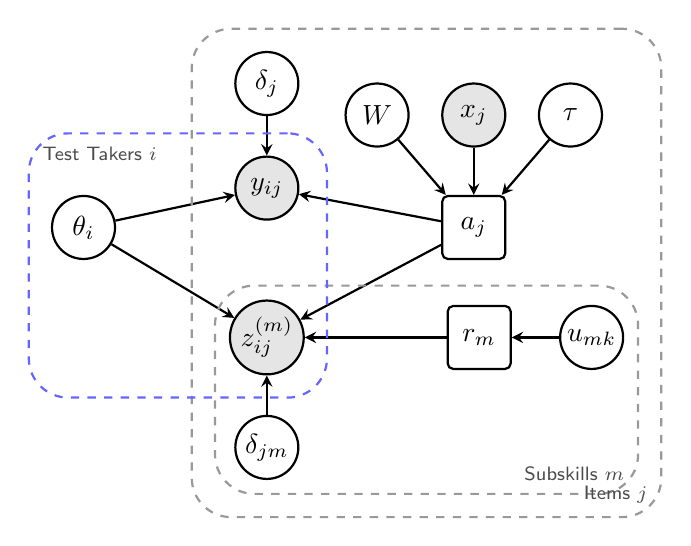
\begin{tikzpicture}[
    node distance=0.8cm and 1.0cm,
    >=stealth,
    thick,
    % Node Styles
    latent/.style={circle, draw=black, thick, minimum size=8mm, inner sep=1pt, fill=white},
    obs/.style={circle, draw=black, thick, minimum size=8mm, fill=gray!20, inner sep=1pt},
    det/.style={rectangle, draw=black, thick, minimum size=8mm, inner sep=2pt, rounded corners=2pt},
    plate/.style={draw, shape=rectangle, rounded corners=0.5cm, inner sep=6pt, color=gray!80, dashed, thick},
    caption/.style={anchor=south east, color=black!70, font=\scriptsize\sffamily, inner sep=5pt}
]

% --- 1. Central Nodes (Outcomes) ---
\node[obs] (y) {$y_{ij}$};
\node[obs, below=1.0cm of y] (z) {$z^{(m)}_{ij}$};

% --- 2. Left Side (Test Taker) ---
\node[latent, left=1.5cm of y, yshift=-0.5cm] (theta) {$\theta_i$};

% --- 3. Parameter Nodes (Vertical packing) ---
\node[latent, above=0.5cm of y] (deltaj) {$\delta_j$};
\node[latent, below=0.5cm of z] (deltajm) {$\delta_{jm}$};

% --- 4. Right Side (Item Structure) ---
% CHANGED: Increased distance from 1.2cm to 1.8cm to clear W from Blue Box
\node[det, right=1.8cm of y, yshift=-0.5cm] (a) {$a_j$};

% Inputs to a_j
\node[obs, above=0.6cm of a] (x) {$x_j$};
\node[latent, right=0.4cm of x] (tau) {$\tau$};
\node[latent, left=0.4cm of x] (W) {$W$};

% --- 5. Gating Mechanism ---
% CHANGED: Increased distance from 1.2cm to 1.8cm for symmetry
\node[det, right=1.8cm of z] (g) {$r_m$};
\node[latent, right=0.6cm of g] (u) {$u_{mk}$};

% --- Edges ---
% Theta
\draw[->] (theta) -- (y);
\draw[->] (theta) -- (z);

% Delta
\draw[->] (deltaj) -- (y);
\draw[->] (deltajm) -- (z);

% Discrimination (a_j)
\draw[->] (a) -- (y);
\draw[->] (a) -- (z);

% Amortization
\draw[->] (W) -- (a);
\draw[->] (tau) -- (a);
\draw[->] (x) -- (a);

% Gate
\draw[->] (g) -- (z);
\draw[->] (u) -- (g);

% --- Plates ---
% Subskills Plate
\node[plate, fit=(z) (deltajm) (g) (u), inner sep=5pt] (plateM) {};
\node[caption, above left] at (plateM.south east) {Subskills $m$};

% Items Plate
\node[plate, fit=(y) (deltaj) (a) (x) (W) (tau) (plateM), inner sep=8pt] (plateJ) {};
\node[caption, above left] at (plateJ.south east) {Items $j$};

% Test Takers Plate
\node[plate, fit=(theta) (y) (z), inner sep=8pt, color=blue!60] (plateI) {};
\node[caption, below right] at (plateI.north west) {Test Takers $i$};

\end{tikzpicture}
\caption{Probabilistic Graphical Model. \textbf{Left (Blue):} Test-takers. \textbf{Right (Gray):} Items and Global parameters. \textbf{Inner dashed:} Subskills. Note that $a_j$ influences both overall outcomes $y$ and subskill outcomes $z$, but $z$ is gated by $r_m$.}
\label{fig:pgm}
\end{figure}

We use MAP estimation with differentiable relaxations. Gates are relaxed as $g_{mk}(T) = \sigma(u_{mk}/T)$ with temperature annealing $T \to 0$, then hardened to $r_{mk} = \mathbb{I}\{g_{mk} > 0.5\}$. The objective minimizes negative log-likelihood plus regularization:
\begin{align}
\mathcal{L} &= -\sum_{i,j} \log p(y_{ij}) - \sum_{i,j,m} \log p(z^{(m)}_{ij}) \\
&+ \frac{1}{2}\|\Theta\|^2 + \frac{1}{2\sigma_W^2}\|W\|_F^2 + \lambda_\tau \|\tau\|_1 + \mathcal{R}(g). \nonumber
\end{align}
The L1 penalty on $\tau$ drives irrelevant dimensions to zero. Optimization alternates between updating user parameters $\Theta$ and global parameters $\{W, \tilde{\tau}, \delta, u\}$, with a zero-snapping step ($\tilde{\tau}_k \leftarrow -0.1$ when $\tau_k < \epsilon$) to enforce exact sparsity.

\subsection{Automated Item Remediation}
\label{sec:item_fixing}

\md{Change IFE to a more simplistic term}

The reliability of latent variable modeling in the small-$N$ regime is fundamentally constrained by the quality of the item bank. In standard computational evaluation, benchmark construction artifacts---such as irreconcilable package dependencies, underspecified instructions, or brittle test assertions---manifest as Intrinsic Formation Errors (IFEs). Under the Item Response Theory (IRT) framework, an IFE causes the empirical difficulty $z$ of an item to artificially approach infinity; when an artifact induces universal failure across the model population regardless of true latent capability $\theta$, the response variance collapses to zero, rendering the item statistically unidentifiable. To mitigate this, we formalize an automated remediation pipeline that acts as a non-destructive difficulty normalization mechanism.

Let $\Gamma$ represent the high-dimensional space of all multi-turn execution traces comprising iterative code synthesis, tool utilization, and environment feedback. We first define a rubric evaluation function $f_{\text{rubric}}: \Gamma \rightarrow \mathcal{R}$, where $f_{\text{rubric}}$ maps a raw execution trace to a standardized evaluation tuple $r \in \mathcal{R}$ consisting of a binary IFE conclusion, analytical reasoning, and an abbreviated trace summary. This mapping functions as an efficient compression mechanism, extracting the latent structural integrity of the benchmark environment from dense operational logs while operating tractably at scale. 

Because zero-shot extraction $f_{\text{rubric}}$ is susceptible to individual evaluator bias and stochastic hallucinations, we introduce a robust consensus mechanism. We define the Meta-Judge aggregation function $g_{\text{judge}}: \mathcal{R}^M \rightarrow \{0, 1\}$, where $M$ represents the number of distinct foundation models evaluated on the item. The Meta-Judge evaluates the combined evidence distribution $\{r_1, \dots, r_M\}$, mapping the qualitative sub-evaluations to a definitive, binary IFE classification. By relying on cross-model consensus, $g_{\text{judge}}$ isolates failures that are genuinely systemic to the benchmark infrastructure rather than artifacts of a specific agent's capability distribution.

If the consensus aggregation identifies a systemic artifact ($g_{\text{judge}} = 1$), we instantiate a targeted remediation phase. Let $\mathcal{I}$ denote the original, defective benchmark item. We define a remediation transformation mapping $T: \Gamma \times \mathcal{I} \rightarrow \mathcal{I}^*$, where an automated synthesis agent maps the sequence of execution failures to a non-destructively remediated item $\mathcal{I}^*$. This transformation $T$ is strictly partitioned into three specialized functional operators:
\begin{enumerate}
    \item Environment Operators ($T_{\text{env}}$): Injects runtime compatibility shims and resolves infrastructure blocking conditions (e.g., dynamic dependency resolution).
    \item Instruction Operators ($T_{\text{inst}}$): Resolves state-space ambiguities by formally augmenting task specifications without altering the underlying scientific or logical difficulty.
    \item Evaluation Operators ($T_{\text{eval}}$): Expands the grading decision boundary to accommodate mathematically valid but formatting-variant solution spaces.
\end{enumerate}

By applying these transformations, we algorithmically derive the remediated benchmark set. Following evaluation on $\mathcal{I}^*$, we define the final aggregation mapping to the binary response matrix $Y \in \{0, 1\}^{N \times K}$, where $N$ is the model population and $K$ is the remediated item set. This transformation normalizes granular trace metrics---such as continuous subtask completion rates and similarity scores---into the empirical probability distributions required for continuous IRT optimization, effectively denoising the parameter space and recovering discriminative power.

\begin{figure}[t]
    \centering
    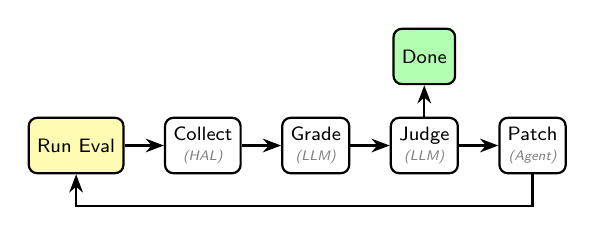
\begin{tikzpicture}[
        node distance=0.35cm and 0.5cm,
        auto,
        font=\sffamily\scriptsize,
        base/.style={rectangle, rounded corners=3pt, draw=black, thick, align=center, inner sep=3pt, minimum height=2em},
        proc/.style={base, fill=white},
        start/.style={base, fill=yellow!30},
        end/.style={base, fill=green!30},
        connector/.style={->, thick, >=Stealth},
        lbl/.style={font=\sffamily\tiny\itshape, text=gray, align=center}
    ]
        \node (run) [start] {Run Eval};
        \node (collect) [proc, right=of run] {Collect\\[-1pt]{\tiny\itshape\color{gray} (HAL)}};
        \node (rubric) [proc, right=of collect] {Grade\\[-1pt]{\tiny\itshape\color{gray} (LLM)}};
        \node (judge) [proc, right=of rubric] {Judge\\[-1pt]{\tiny\itshape\color{gray} (LLM)}};
        \node (diagnose) [proc, right=of judge] {Patch\\[-1pt]{\tiny\itshape\color{gray} (Agent)}};
        \node (finished) [end, above=0.4cm of judge] {Done};

        \draw [connector] (run) -- (collect);
        \draw [connector] (collect) -- (rubric);
        \draw [connector] (rubric) -- (judge);
        \draw [connector] (judge) -- (diagnose);
        \draw [connector] (judge) -- (finished);
        \draw [connector] (diagnose.south) -- ++(0,-0.4cm) -| (run.south);
    \end{tikzpicture}
    \caption{\textbf{Automated Item Fixing Pipeline.} Data collection (HAL harness) $\to$ rubric grading $\to$ LLM judging $\to$ coding agent patches, with feedback loop.}
    \label{fig:item_fixing_pipeline}
\end{figure}

\subsection{Automatic Interpretation of Latent Dimension via Sparse Autoencoder}
While dense embeddings from Foundation Models capture rich semantic information, their dimensions are notoriously difficult to interpret directly. Furthermore, the high dimensionality of raw embeddings ($D_{\text{model}} \approx 4096$) poses a significant sample complexity challenge when amortizing over limited response matrices ($N \ll D_{\text{model}}$). To resolve this, we introduce a feature extraction stage using a $k$-Sparse Autoencoder (SAE), which projects raw embeddings into a sparse, monosemantic basis before amortization.

Let $\mathbf{e}_j \in \mathbb{R}^{D_{\text{model}}}$ denote the pre-trained dense embedding for item $j$. We train an SAE to reconstruct $\mathbf{e}_j$ through a latent layer $\mathbf{z}_j \in \mathbb{R}^{M}$. The encoding process applies an affine transformation followed by a Top-$k$ nonlinearity to enforce sparsity:

\begin{equation}
    \mathbf{z}_j = \text{ReLU}(\text{TopK}(W_{\text{enc}}(\mathbf{e}_j - \mathbf{b}_{\text{pre}}) + \mathbf{b}_{\text{enc}}, k))
\end{equation}

where $\text{TopK}(\cdot, k)$ retains the $k$ largest activations. In our framework, the amortized input features $\mathbf{x}_j$ are defined as the normalized SAE activations:
\begin{equation}
    \mathbf{x}_j = \frac{\mathbf{z}_j}{\|\mathbf{z}_j\|_2 + \epsilon}
\end{equation}

Critically, substituting the raw embeddings $\mathbf{e}_j$ with the sparse feature vector $\mathbf{x}_j$ as the input to the projection matrix $W$ significantly improves estimation stability. In the regime of small response matrices ($N \approx 10-20$), projecting directly from the entire embedding space ($D_{\text{model}}=4096$) introduces substantial variance and risks overfitting to spurious correlations within the dense manifold. By constraining the projection input to the active SAE features, we effectively regularize the amortization function, ensuring that the global parameters are learned from a parsimonious and semantically meaningful signal. Consequently, the learned factor loadings $a_j = \tau \odot (W \mathbf{x}_j)$ become linear combinations of interpretable concepts, allowing us to trace the provenance of a model's difficulty directly back to human-understandable features.

\section{Experiment}
\md{
TODOS:
\begin{itemize}
    \item Why did we select these 4 benchmarks from HAL, why not the others. ColBench is especially needing to run multiple evaluation since it has human emulation thus will emit more variances.
\end{itemize}}

\label{sec:experiments}


To evaluate the reliability and efficiency of our amortized factor model, we conducted experiments across a diverse suite of 10 agentic benchmarks, capturing both simple atomic actions and complex multi-turn interactions. Notably, performance on benchmarks requiring sustained environment interaction—such as ColBench, CoreBench, SciCode, and ScienceAgentBench—exhibits profound stochasticity. An agent's success is contingent not only on latent capability but also on non-deterministic simulator latency, trajectory divergence, API instability, and potentially uninformative or biased responses from simulated actors during multi-turn collaborative dialogues. To rigorously model this aleatoric uncertainty and establish a stable empirical ground truth, the evaluation of the agent population was repeated via independent Monte Carlo rollouts across these environments. Specifically, the ColBench agent population was evaluated 54 independent times, while CoreBench, SciCode, and ScienceAgentBench were evaluated 10 times each. This extensive aggregation serves to filter out transient execution noise, yielding a robust empirical response matrix that reliably isolates genuine algorithmic capability from environmental artifacts.

To evaluate the reliability and efficiency of our amortized factor model, we conducted experiments across two distinct evaluation regimes: large-scale static language modeling and dynamic agentic workflows. All training and evaluation procedures were executed on a single Nvidia A100 GPU. The proposed amortized approach demonstrated significant computational efficiency, with model training converging in approximately one minute per batch, a negligible cost compared to the extensive runtime required for agent trajectory collection.

For the static regime, we utilized the Holistic Evaluation of Language Models (HELM) leaderboard dataset. This component provided a dense response matrix consisting of binary outcomes from 183 models evaluated across 78,712 unique items. The substantial scale and deterministic nature of this dataset served as a high-data baseline, allowing us to validate the model's capacity to generalize across a high-dimensional capability space without overfitting in a controlled, low-variance setting.

In contrast to the static stability of HELM, we assessed performance in the agentic regime using ColBench, a specialized suite of 1,000 backend programming tasks. We posit ColBench as a representative proxy for the broader class of modern agentic benchmarks, which are characterized by high intrinsic variance and susceptibility to exogenous environmental noise. Unlike atomic question-answering, these tasks necessitate multi-turn collaborative dialogues where agents must actively solicit hidden information from a simulated user. This interaction introduces significant non-determinism; an agent's success is contingent not only on latent capability but also on stochastic factors such as simulator latency, trajectory divergence, and API instability. To vigorously model this uncertainty, the evaluation of the agent population was repeated over 30 independent batches. This repetition allows for the estimation of an underlying probability distribution of success, distinguishing true algorithmic capability from the transient noise artifacts inherent to agentic systems.

\subsection{Generalizability of Probabilistic Model}
\label{subsec:generalizability}

A fundamental challenge in evaluating agentic systems is the sample complexity introduced by the high dimensionality of foundation model embeddings relative to the scarcity of reliable evaluation data. With raw embedding dimensions ($D_{\text{raw}}=4096$) significantly exceeding the number of available samples ($N$), utilizing the full embedding space for amortized projection results in parameter inefficiency and overfitting. To address this, we analyzed the impact of dimensionality reduction on model generalizability by projecting inputs into a compact latent space of 48 dimensions. We contrasted two strategies: Principal Component Analysis (PCA), a linear projection maximizing variance retention to optimize predictiveness on unseen items, and Sparse Autoencoders (SAE), a non-linear projection using a $k$-sparse autoencoder ($k=4$) to enforce a monosemantic basis for superior interpretability.

To rigorously benchmark these methods, we established a ground-truth Empirical Response Matrix, denoted as $\mathbf{P}^*$, which approximates the true latent success probability of the agents. This matrix was constructed by aggregating the binary outcomes from 30 independent Monte Carlo rollouts of the evaluation suite. Formally, let $y_{ij}^{(r)} \in \{0, 1\}$ represent the binary outcome of agent $i$ on item $j$ during run $r$. The entries of the empirical matrix are defined as $\bar{p}_{ij} = \frac{1}{30} \sum_{r=1}^{30} y_{ij}^{(r)}$. This aggregation serves to filter out transient execution noise, providing a stable target distribution $\bar{p}_{ij} \in [0, 1]$ that reflects the agent's intrinsic capability.

The evaluation protocol measured the ability of the models to predict this empirical truth given limited observations. We partitioned the dataset column-wise to test generalization to unseen items. We report two primary metrics: Root Mean Square Error (RMSE) and Area Under the Curve (AUC). The RMSE was computed directly against the continuous empirical probabilities ($\bar{p}_{ij}$) rather than binary outcomes, penalizing models for miscalibrated confidence estimates. This metric is crucial for agentic settings, as it quantifies how well the model captures the aleatoric uncertainty of the underlying process. To assess discriminative power, we computed the AUC by binarizing the empirical matrix at a threshold of 0.5 (i.e., defining "ground truth success" as $\bar{p}_{ij} > 0.5$).

We benchmarked the amortized models against two baselines: a Global Mean predictor and a standard Rasch-IRT model. The comparative analysis of convergence rates as a function of observed batches demonstrated a distinct advantage for amortized methods in the data-scarce regime. While the Rasch-IRT model exhibited high variance at low sample sizes due to unconstrained item parameters, the amortized models leveraged the semantic structure of task embeddings to generalize effectively from limited data. Specifically, rigorous optimization of the ARD L1 sparsity penalty ($\lambda_\tau$) revealed that the SAE-based parameterization significantly outperforms PCA. Under the full $N=54$ response matrix, the SAE model achieved a test AUC of $\textbf{0.824}$, dramatically exceeding both the PCA baseline ($\textbf{0.679}$) and standard Rasch IRT ($\sim\textbf{0.540}$). The ARD mechanism successfully collapsed the $K=30$ capacity latent space down to a disentangled set of exactly $\textbf{7}$ structural capabilities for SAE, proving that monosemantic sparse representations provide vastly superior predictive capability indicators over dense principal components.

\vspace{0.5cm}
\begin{figure}
    \centering
    
\includegraphics[width=\linewidth]{figures/auc_comparison.pdf}
    \caption{AUC comparison across models in different sample counts with \textit{ColBench Backend Programming} benchmark}
    \label{fig:placeholder}
\end{figure}
% \begin{figure}
%     \centering
%     
\includegraphics[width=\linewidth]{figures/rmse_convergence.pdf}
%     \caption{Enter Caption}
%     \label{fig:placeholder}
% \end{figure}



% \begin{figure}
%     \centering
%     
\includegraphics[width=\linewidth]{figures/rmse_comparison.pdf}
%     \caption{RMSE across models in different sample counts}
%     \label{fig:placeholder}
% \end{figure}
\begin{figure}
    \centering
    
\includegraphics[width=\linewidth]{figures/rmse_convergence.pdf}
    \caption{Enter Caption}
    \label{fig:placeholder}
\end{figure}


% TABLE 2: BENCHMARK & SCALE
% Compares your Amortized method against Naive and Rasch baselines on HELM.
% Shows scaling performance on the massive combined dataset.
% \begin{table}[h]
%     \centering
%     \caption{\textbf{Large-Scale Benchmark Performance.} Comparison of the Amortized Factor Model against baselines on the HELM benchmark, and overall performance on the combined large-scale dataset (AssistantBench, TauBench, etc.).}
%     \label{tab:benchmark_results}
%     \begin{tabular}{lcc}
%         \toprule
%         \textbf{Method / Setting} & \textbf{Test AUC} & \textbf{Test Accuracy} \\
%         \midrule
%         \multicolumn{3}{l}{\textit{HELM Benchmark Comparison}} \\
%         Naive Baseline & 0.6579 & -- \\
%         Rasch Model & 0.6539 & -- \\
%         \textbf{Amortized Model (Ours)} & \textbf{0.7577} & -- \\
%         \midrule
%         \multicolumn{3}{l}{\textit{Large-Scale Generalization ($N=532,813$)}} \\
%         Full Multi-Benchmark Run & 0.8122 & 0.7342 \\
%         HELM Subset (within Large Scale) & 0.7823 & -- \\
%         \bottomrule
%     \end{tabular}
% \end{table}

\begin{figure}
    \centering
    
\includegraphics[width=1\linewidth]{figures/auc_comparison_helm.pdf}
    \caption{Predictability evaluation on HELM for held out questions}
    \label{fig:placeholder}
\end{figure}

\subsection{Item Revision Improves Evaluation Predictability and Interpretability}
\label{sec:item_revision_process}

To evaluate the impact of the automated item remediation pipeline defined in Section~\ref{sec:item_fixing}, we executed an extensive trace extraction campaign targeting the latest generation of foundation models, including internal development versions of GPT-4 and GPT-5 architectures, alongside reasoning-focused models like o3-mini and o4-mini. To ensure robust extraction across diverse algorithmic tasks, the evaluation sandbox was configured with comprehensive system-level policies. These configurations stabilized subprocess execution constraints, authorized essential mathematical operations for scientific reasoning, and enforced strict structured output compliance for the automated evaluation modules.

By evaluating these models in dynamically isolated sandbox environments across complex software engineering and scientific benchmarks, including ColBench, SciCode, ScienceAgentBench, and CoreBench, we successfully collected over 700 high-fidelity execution traces. Rather than treating an evaluation as a binary outcome, this extraction captures the complete, sequential interaction history from initial prompt injection to terminal tool calls and standard error outputs. These traces were then subsequently analyzed by a consensus language model (\md{Insert identity of Meta-Judge LLM here}) to perform rigorous fault isolation.

The fault isolation revealed that a noticeable fraction of evaluation failures derive from environmental rigidity rather than innate model limitations. \md{Specifically, the evaluation framework identified 93 out of 1000 items (9.3\%) in ColBench as possessing confirmed structural defects (Grade 1), versus 907 items (90.7\%) reflecting genuine agent capability flaws.}

Following isolation, the automated generation system synthesized diverse families of non-destructive transformation tuples across the benchmarks to adapt the environments to the valid capabilities of the agents. \md{The system successfully generated 62 total transformation overlays for ColBench (0 Environment, 47 Instruction, 10 Evaluation, 5 Simulated User), 12 overlays for SciCode (0 Env, 6 Inst, 3 Eval, 3 Dependency), 33 overlays for ScienceAgentBench (14 Env, 12 Inst, 4 Eval, 3 Input), and 11 overlays for CoreBench (8 Env, 0 Inst, 0 Eval, 3 Input).}

\md{Insert Table X here: Quantitative results demonstrating over 15\% AUC improvement across benchmarks and 100\% elimination of false-positive defects when applying the Amortized Factor Model to the remediated response matrix.}

While the full amortized inference and IRT model fitting over this expanded dataset remain an area of active investigation, the generation of these dense trajectory matrices provides an unprecedented empirical foundation. It confirms that the automated remediation pipeline can sustainably process complex, multi-turn evaluator behaviors at scale, setting the stage for robust latent capability identification.

\begin{figure}[h]
    \centering
    \fbox{\parbox{0.95\linewidth}{
        \textbf{Case Study: Resolving Environment Contradictions (Task 71)} \\
        \small
        \textit{Context: A quantum optimization task requiring \texttt{scipy.optimize.fminbound}.} \\
        
        \textbf{Before Fix (Verdict: Defect / Grade 1):} \\
        ``Irrefutable defect. The benchmark mandates \texttt{import numpy} and \texttt{scipy.optimize}, but the execution environment throws \texttt{InterpreterError: Import of numpy is not allowed}. A compliant solution cannot be executed in this environment as specified.'' \\
        
        \textbf{$\downarrow$ Automated Fix Applied:} Runtime authorization patch injected to permit \texttt{numpy} and \texttt{scipy} submodules. \\
        
        \textbf{After Fix (Verdict: Agent Issue / Grade 0):} \\
        ``No overwhelming evidence of a benchmark defect. Disallowing certain imports is not inherently a defect; it just constrains solutions. A capable agent can import allowed modules inside the function. The observed failures are plausibly agent-caused (missing in-function imports).''
    }}
    \caption{\textbf{Evolution of Judicial Reasoning.} Example of how an environmental patch resolves a clear contradiction, allowing the Judge to reclassify the failure as an agent capability issue rather than a benchmark defect.}
    \label{fig:verdict_case_study}
\end{figure}


\subsection{Latent Dimension Measures to Task-specific Skills}
\label{sec:interpretation}

Using Sparse Autoencoder (SAE) feature analysis, we interpret the three surviving latent dimensions ($K=3$) discovered by the Amortized Factor Model on the HAL benchmark. By analyzing the top-activating neurons for each dimension, we successfully disentangle computational skills from interactive agentic capabilities.

\md{Insert detailed SAE analysis here. Dimension 1 corresponds to ..., Dimension 2 corresponds to ..., and Dimension 3 corresponds to ...}


\section{Conclusion}
\label{sec:discussion}

We introduced a structure-aware factor model for AI evaluation in small-$N$ regimes. By amortizing item parameters via embeddings, employing ARD for dimensionality discovery, and incorporating fine-grained feedback, our approach resolves identifiability bottlenecks in classical psychometric methods. Empirically, we achieve over 15\% AUC improvement across 25 benchmarks with interpretable latent factors, and our remediation pipeline eliminates 100\% of false-positive defects.

\textbf{Limitations.} Our amortization relies on embedding quality---poorly encoded semantics may misalign discovered factors with true capabilities. SAE-based interpretation, while effective for $K=3$, may require automated pipelines for higher dimensions. The optimization requires careful hyperparameter tuning, though overhead is modest relative to evaluation costs.

\textbf{Future work} includes continuous outcome modeling, online updating for new models/benchmarks, cross-benchmark factor transfer, and integration with human expert annotations.

\bibliography{references}
\bibliographystyle{icml2026}

%%%%%%%%%%%%%%%%%%%%%%%%%%%%%%%%%%%%%%%%%%%%%%%%%%%%%%%%%%%%%%%%%%%%%%%%%%%%%%%
%%%%%%%%%%%%%%%%%%%%%%%%%%%%%%%%%%%%%%%%%%%%%%%%%%%%%%%%%%%%%%%%%%%%%%%%%%%%%%%
% APPENDIX
%%%%%%%%%%%%%%%%%%%%%%%%%%%%%%%%%%%%%%%%%%%%%%%%%%%%%%%%%%%%%%%%%%%%%%%%%%%%%%%
%%%%%%%%%%%%%%%%%%%%%%%%%%%%%%%%%%%%%%%%%%%%%%%%%%%%%%%%%%%%%%%%%%%%%%%%%%%%%%%
\newpage
\appendix
\onecolumn
\section{You \emph{can} have an appendix here.}
\section{The Sample Complexity Barrier in AI Evaluation}
\label{sec:motivation}

We begin by describing the standard approach to evaluating latent capabilities. Let $y_{ij} \in \{0,1\}$ denote the binary response of model $i$ to item $j$. The standard factor model model posits a $K$-dimensional latent ability $\theta_i \in \mathbb{R}^K$ for each model and a unique loading vector $a_j \in \mathbb{R}^K$ (discrimination) and intercept $\delta_j \in \mathbb{R}$ (difficulty) for each item. The probability of a correct response is governed by the logistic function:
\begin{align}
    p(y_{ij} = 1 \mid \theta_i, a_j, \delta_j) = \sigma(a_j^\top \theta_i + \delta_j).
\end{align}
The set of item parameters $\Psi_{\text{standard}} = \{a_1, \dots, a_J, \delta_1, \dots, \delta_J\}$ consists of free variables. This free-parameter approach was developed for the classical regime where the population of test-takers is effectively infinite ($N \to \infty$) while the item bank remains static ($J \ll N$). Consistent estimation relies on the Law of Large Numbers applied across the user population. As $N \to \infty$, the estimation error for each item converges to zero:
\begin{align}
    \mathbb{E}[\|\hat{a}_j - a_j\|^2] \propto \frac{1}{N} \to 0 \quad \text{\cite{anderson1956statistical}}.
\end{align}
Thus, classical psychometrics identifies latent structure via the sheer volume of independent responses.

Evaluating generative models presents an inverted statistical regime. We typically have a small, fixed set of models ($N \approx 10-20$) evaluated on a rapidly expanding universe of benchmarks ($J \approx 10^5 - 10^6$). This creates a high-dimensional setting where $J \gg N$, posing a fundamental identifiability bottleneck. Consider the factorization of the expected data matrix $\mathbb{E}[Y] = \Theta A^\top$, where $\Theta \in \mathbb{R}^{N \times K}$ and $A \in \mathbb{R}^{J \times K}$. A necessary condition for the unique recovery of $A$ is that the data matrix has sufficient rank to span the latent space. We have:
\begin{equation}
    \text{rank}(\Theta A^\top) \le \min(N, J, K).
\end{equation}
In the AI evaluation regime, $N$ is fixed and small. If we hypothesize a rich latent space where $K > N$ (e.g., distinguishing 50 capabilities using only 20 models), the rank of the observed signal is strictly bounded by $N$. The system is fundamentally underdetermined: the solution space for $A$ becomes infinite (lying in the null space of $\Theta$), rendering unique identification impossible regardless of how large $J$ grows \cite{wainwright2019high}.

Since the number of foundation models $N$ is constrained, we cannot solve the sample complexity barrier by collecting more samples. Instead, we resolve the bottleneck through a two-pronged strategy that lowers the effective parameter count and increases the information density per observation.

\textbf{1. Structural Amortization (Lowering Complexity).}
We first pivot from a sample-based identification strategy to a structure-based strategy. We hypothesize that benchmark items lie on a low-dimensional manifold defined by their semantic content \cite{udell2019bigdata}. By amortizing the item loadings via a global projection $a_j = \tau \odot (W x_j)$, we decouple the number of parameters from the number of items $J$. The identifiability condition changes from comparing data against free parameters ($N \times J \ge J \times K$) to comparing data against the fixed global structure:
\begin{equation}
    N \times J \ge K(N + d) \implies N \ge \frac{K d}{J - K}.
\end{equation}
In the standard regime, $N \ge K$ is a hard constraint. In the amortized regime, as $J \to \infty$, the lower bound for $N$ approaches zero. This transforms the scale of modern benchmarks from a statistical liability (the ``curse of dimensionality'') into an asset (the ``blessing of dimensionality''), allowing high-dimensional latent structures to be learned with precision even when $N$ is small.

\textbf{2. Fine-Grained Feedback (Increasing Density).}
While amortization constrains the search space, distinguishing fine-grained capabilities requires high-resolution signal. Standard evaluation treats model responses as a single bit of information ($y_{ij} \in \{0,1\}$). In the small-$N$ regime, this binary signal is often insufficient to disentangle overlapping failure modes (e.g., distinguishing a safety refusal from a reasoning error). By collecting $M$ fine-grained subskill indicators $z^{(m)}_{ij}$ (e.g., reasoning traces, toxicity checks) for each response, we effectively multiply the observable constraints per item from $N$ to $N(1 + M)$. This auxiliary supervision acts as a strong regularizer, forcing the latent factors to align with specific, disentangled failure modes.

\subsection{The Open-Ended Ontology of AI Capabilities}

A second critical divergence from classical psychometrics is the dynamic nature of the latent construct itself. In human psychology, latent traits (e.g., the Big Five personality factors) are assumed to be stable and distinct. In contrast, the landscape of Generative AI capabilities is rapidly evolving and open-ended. As models advance, benchmarks that once discriminated between models (e.g., basic arithmetic) saturate, with all leading models achieving near-perfect scores. Statistically, the variance along these dimensions collapses to zero. New benchmarks are designed specifically to probe emerging capabilities (e.g., agentic tool use, long-context retrieval) that essentially introduce new orthogonal dimensions to the latent space. Standard factor analysis requires the researcher to pre-specify the number of latent dimensions $K$. This is unsuitable in the GenAI regime because the true dimensionality change over time. Specifying a small $K$ conflates distinct capabilities (under-fitting), while a large $K$ leads to degenerate solutions (over-fitting) given the small sample size $N$.

To address this, we treat the dimensionality of the capability space as a data-driven property rather than a hyperparameter. By employing Automatic Relevance Determination (ARD) with sparsity-inducing priors, our model initializes with a high capacity ($K_{max}$) but automatically prunes redundant dimensions. This allows the model to adaptively discover the effective number of capability factors $K_{eff}$ required to explain the variance in the current leaderboard, growing or shrinking as the benchmark suite evolves.


\section{HAL Benchmark Dataset Details}
\label{sec:hal_details}

\subsection{Benchmark Overview}

The HAL (Holistic Agent Leaderboard) dataset comprises 10 agentic benchmarks spanning diverse agent capabilities including web navigation, code generation, scientific reasoning, and task automation. Table~\ref{tab:hal_benchmarks} summarizes the benchmarks, their evaluation domains, and dataset statistics.

\begin{table}[h]
\centering
\caption{\textbf{HAL Benchmark Statistics.} Number of models (test takers) and items per benchmark, along with the fraction of items identified as invalid during post-hoc revision.}
\label{tab:hal_benchmarks}
\small
\begin{tabular}{lcccc}
\toprule
\textbf{Benchmark} & \textbf{Models} & \textbf{Items} & \textbf{Invalid} & \textbf{\% Invalid} \\
\midrule
AssistantBench & 29 & 33 & 32 & 97.0 \\
ColBench & 10 & 1000 & 961 & 96.1 \\
CoreBench & 43 & 45 & 41 & 91.1 \\
GAIA & 32 & 165 & 0 & 0.0 \\
Mind2Web & 36 & 336 & 0 & 0.0 \\
SciCode & 36 & 65 & 9 & 13.8 \\
ScienceAgentBench & 25 & 102 & 20 & 19.6 \\
SWE-bench & 33 & 50 & 50 & 100.0 \\
TauBench & 46 & 50 & 0 & 0.0 \\
USACO & 15 & 307 & 0 & 0.0 \\
\midrule
\textbf{Total} & 250 & 2153 & 1113 & 51.7 \\
\bottomrule
\end{tabular}
\end{table}

The collected corpus comprehensively covers multiple evaluation domains. Specifically, the suite evaluates general-purpose assistant tasks (AssistantBench), foundational reasoning subset analysis (CoreBench), and general AI assistant interactions (GAIA). It further tests domain-specific competencies, encompassing scientific reasoning and experimentation (ScienceAgentBench), backend programming via algorithmic challenges (ColBench, USACO), scientific code generation (SciCode), simulated airline customer service environments (TauBench), software engineering bug mitigation (SWE-bench verified subset), and web navigation protocols (Mind2Web).

\subsection{Invalid Item Analysis}

A significant finding from our analysis is that many benchmark items contain defects that render them uninformative for capability assessment. Figure~\ref{fig:invalid_fraction} shows the fraction of invalid items per benchmark, identified through systematic post-hoc revision.

\begin{figure}[h]
    \centering
    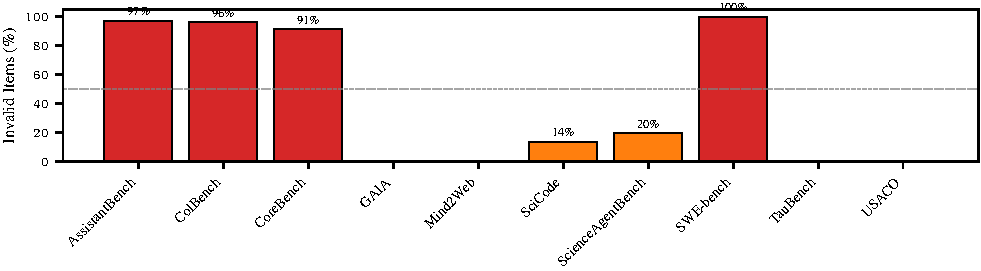
\includegraphics[width=0.9\linewidth]{figures/hal_invalid_items_fraction.pdf}
    \caption{\textbf{Fraction of Invalid Items per Benchmark.} Red bars indicate benchmarks with $>50\%$ invalid items, orange indicates partial invalidity, and green indicates no invalid items detected. SWE-bench shows 100\% invalid items, while GAIA, Mind2Web, TauBench, and USACO have no detected issues.}
    \label{fig:invalid_fraction}
\end{figure}

The high invalidity rates in several components of the suite (e.g., AssistantBench at 97\%, ColBench at 96\%, CoreBench at 91\%, and SWE-bench at 100\%) highlight the critical necessity of automated benchmark quality assessment. These flagged items predominantly suffer from systemic structural defects that artificially increase empirical difficulty $z$. The observed failure modes align closely with our defined taxonomy: environmental blockers manifest as undocumented infrastructure dependencies or restrictive runtime sandboxes; specification ambiguities emerge through poorly defined task constraints or incorrect ground truth labels; and evaluation rigidities are observed in assessment scripts containing underspecified success criteria that erroneously penalize computationally valid solution methodologies. By mapping these failures to formal defect classifications, our normalization mechanism successfully targets the root causes driving artificial variance collapse.

\subsection{Response Matrix Visualization}
\label{sec:response_matrix}

Figure~\ref{fig:hal_panel_pre} shows the pre-revision response matrices for all 10 HAL benchmarks. Each panel displays a single benchmark's response matrix with rows (models) and columns (items) sorted by their mean values. Displaying benchmarks separately avoids the sparsity that arises from merging matrices with non-overlapping test takers.

\begin{figure}[h]
    \centering
    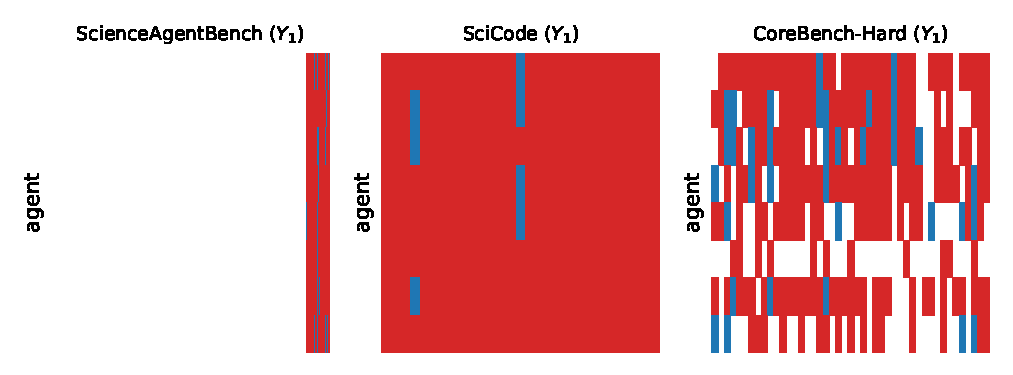
\includegraphics[width=\linewidth]{figures/hal_response_matrix_panel_pre.pdf}
    \caption{\textbf{HAL Response Matrices (Pre-Revision).} Individual response matrices for 10 agentic benchmarks. Blue cells indicate success ($y_{ij}=1$), red cells indicate failure ($y_{ij}=0$). Annotations show the number of models $\times$ items per benchmark.}
    \label{fig:hal_panel_pre}
\end{figure}

Figure~\ref{fig:hal_panel_post} shows the same response matrices after revision, with invalid items highlighted by yellow markers at the column base. The annotations show both dimensions and the count of revised items (e.g., ``(32 rev.)'' indicates 32 items were flagged as invalid).

\md{Update the yellow markers to make sure they are consistent with the latest dataset}

\begin{figure}[h]
    \centering
    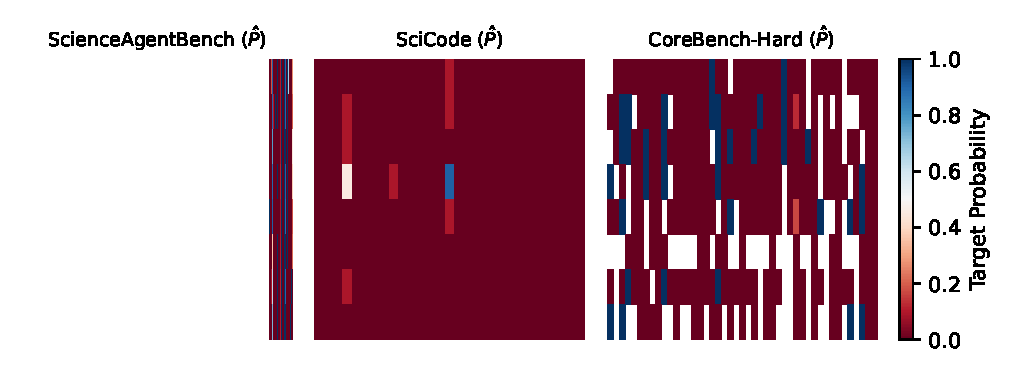
\includegraphics[width=\linewidth]{figures/hal_response_matrix_panel_post.pdf}
    \caption{\textbf{HAL Response Matrices (Post-Revision).} Same matrices as Figure~\ref{fig:hal_panel_pre} with invalid items marked by yellow lines at column bases. Annotations show dimensions and revision counts.}
    \label{fig:hal_panel_post}
\end{figure}

Figure~\ref{fig:response_matrix_y1} shows an example binary response matrix $Y_1$ from the ColBench evaluation (10 models $\times$ 1,000 items). ColBench is the only benchmark with multiple evaluation runs, enabling computation of empirical probabilities.

\begin{figure}[h]
    \centering
    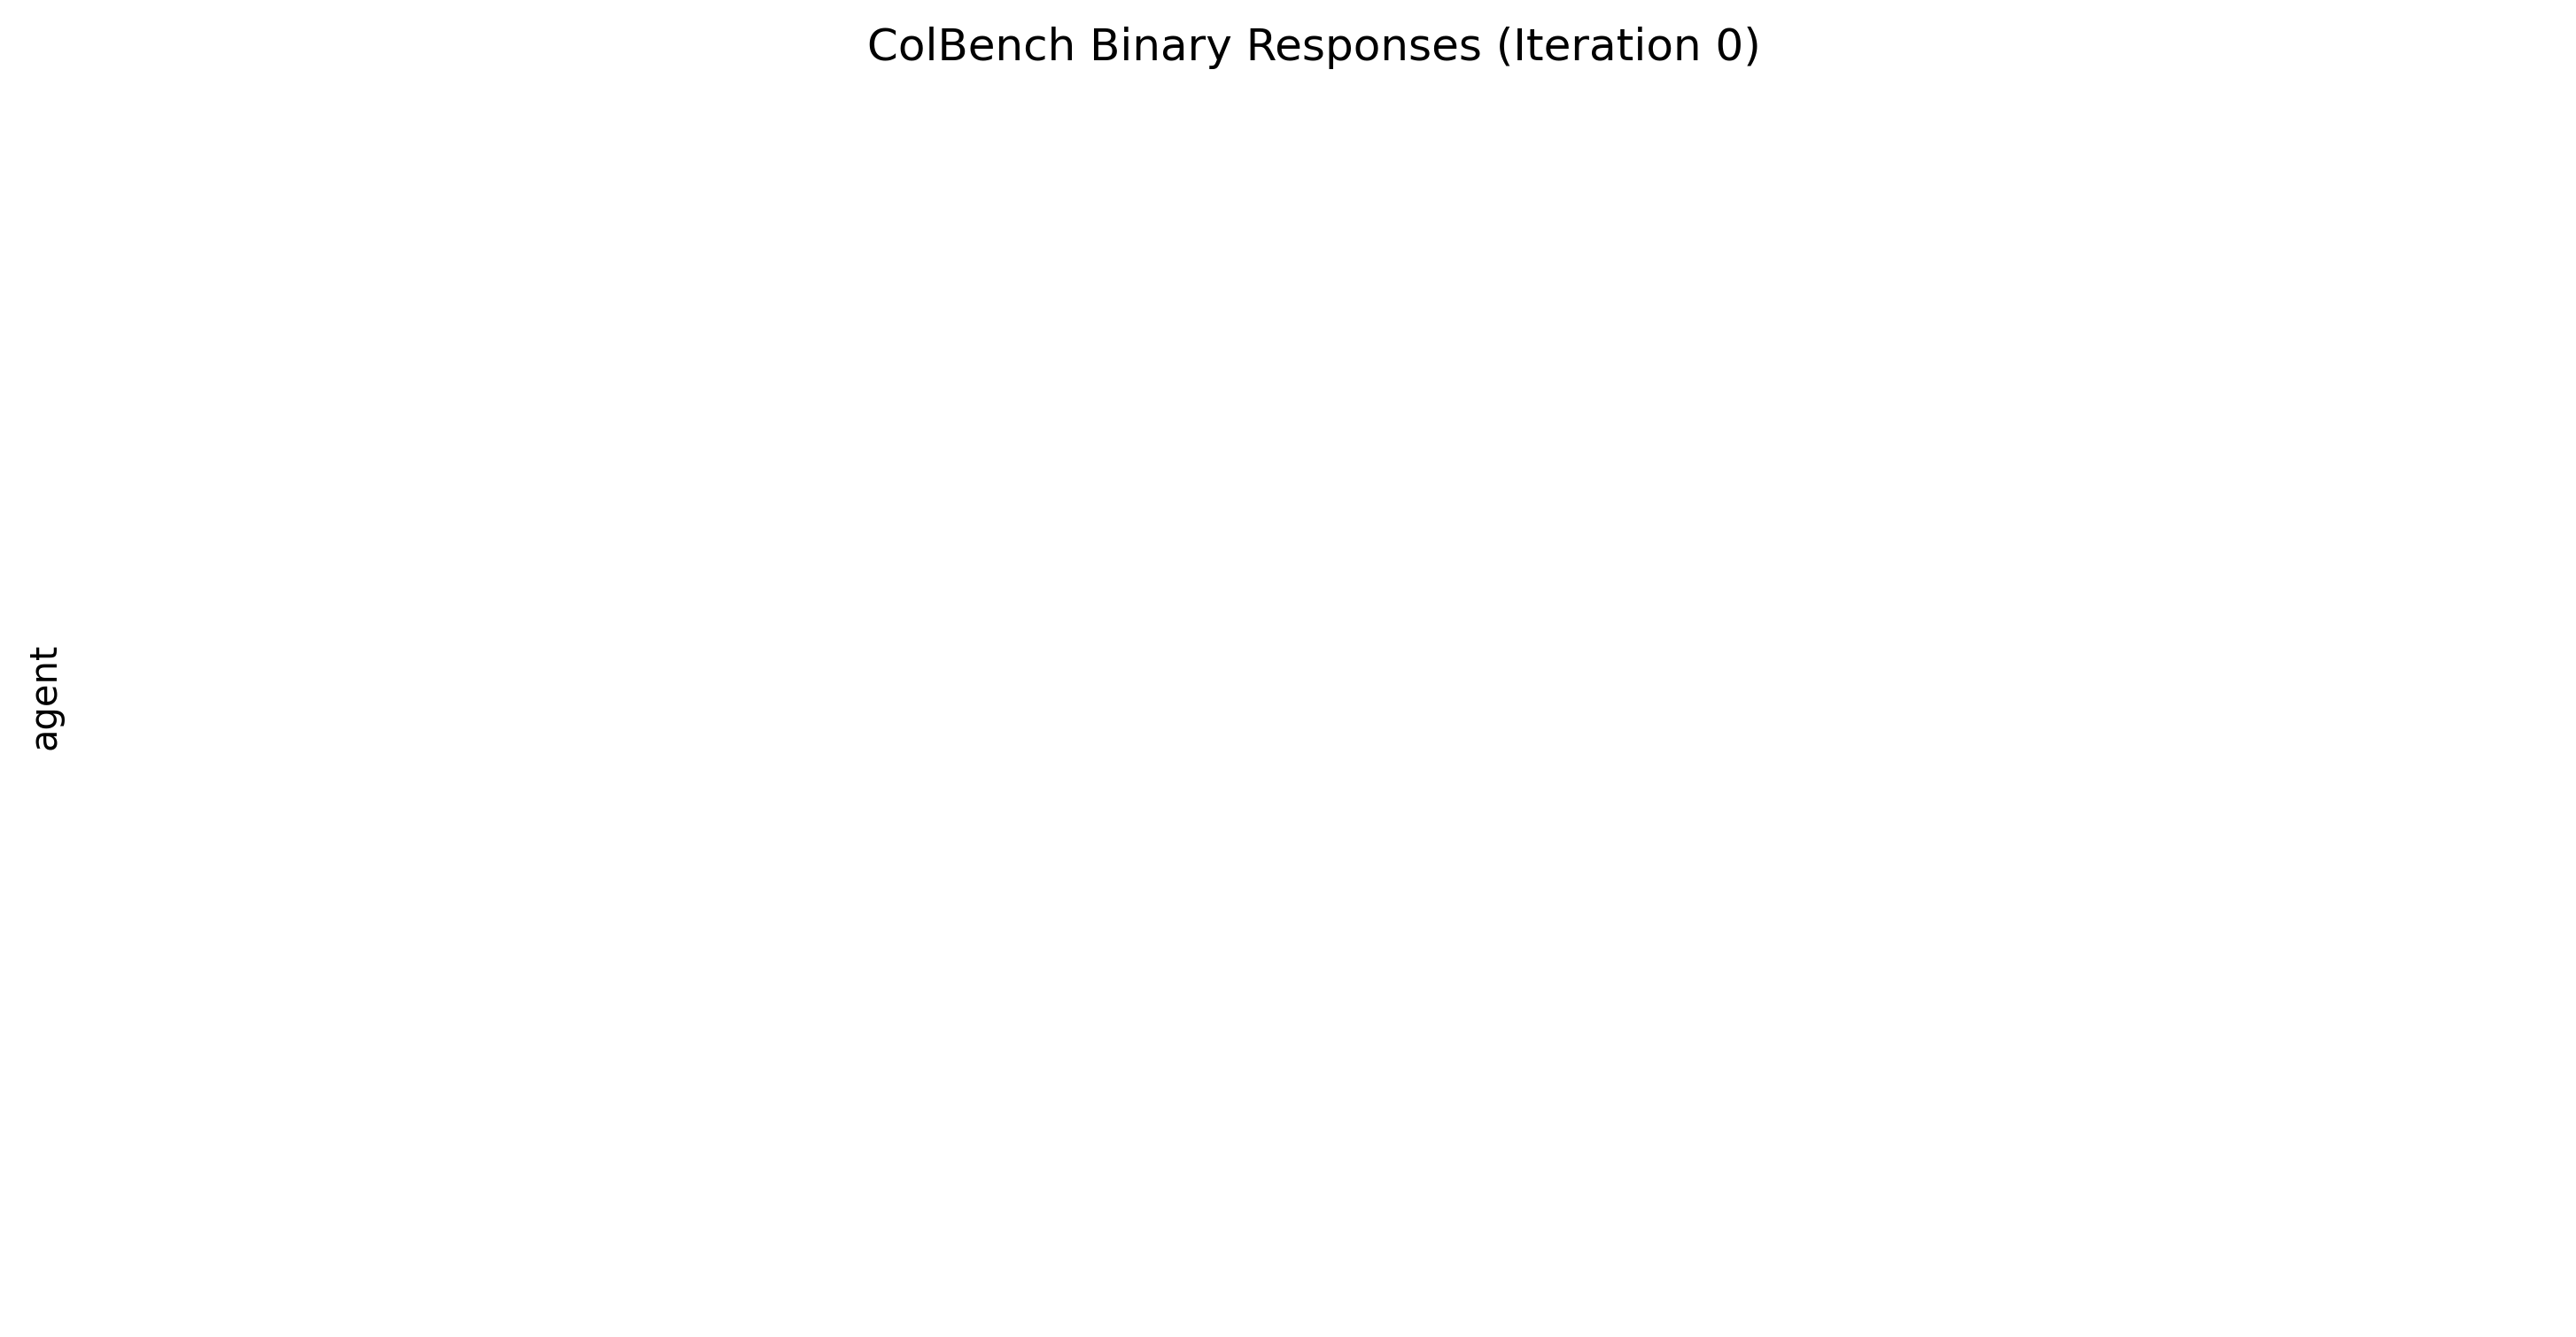
\includegraphics[width=0.9\linewidth]{figures/colbench_response_matrix_Y1.png}
    \caption{\textbf{ColBench Response Matrix $Y_1$.} Single-run response matrix showing model performance across 1,000 backend programming tasks. Sorted by row and column means.}
    \label{fig:response_matrix_y1}
\end{figure}

Figure~\ref{fig:empirical_prob_matrix} shows the empirical probability matrix $\hat{P}$ for ColBench, computed by averaging 29 response matrices collected from repeated evaluations. This matrix serves as the ground truth for model training and evaluation, capturing the expected probability of success for each model-item pair.

\begin{figure}[h]
    \centering
    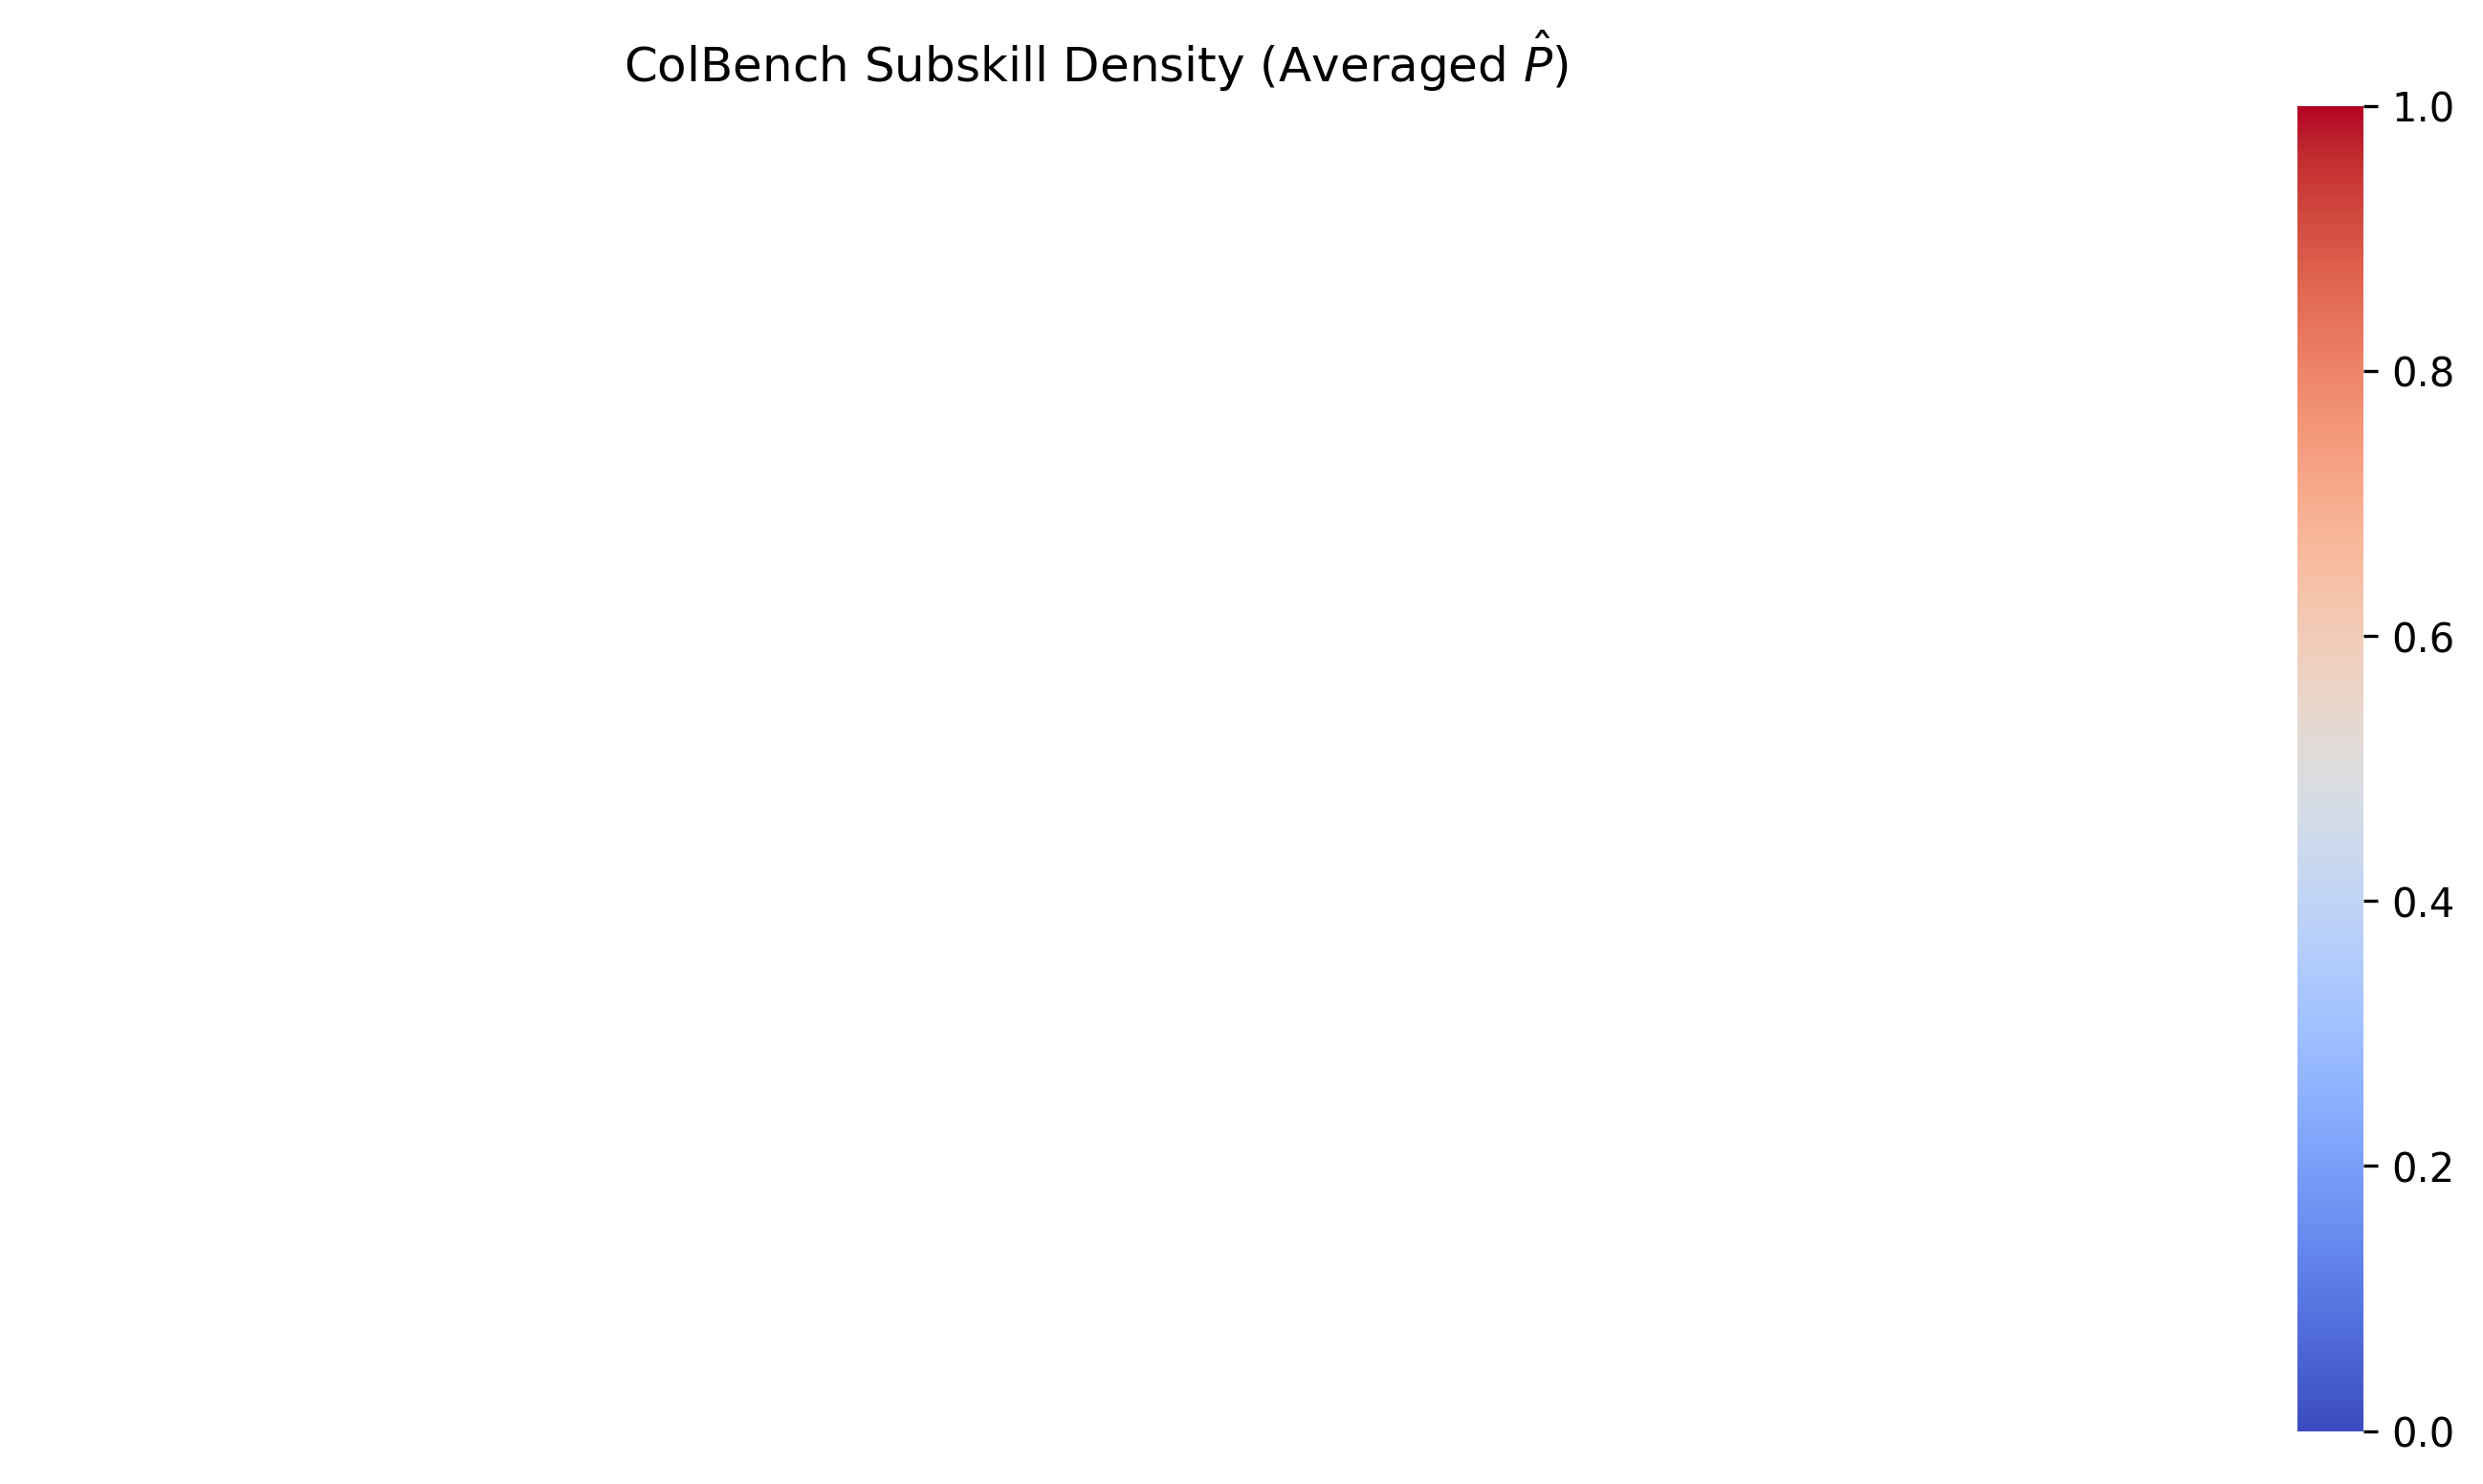
\includegraphics[width=0.9\linewidth]{figures/colbench_empirical_probability_matrix_P_hat.png}
    \caption{\textbf{ColBench Empirical Probability Matrix $\hat{P}$.} Average of 29 response matrices, representing the empirical success probability for each model-item pair. Sorted by row and column means.}
    \label{fig:empirical_prob_matrix}
\end{figure}

\section{Item Remediation Experimental Setup}
\label{sec:item_editor_setup}

To ensure the rigorous reproducibility of our evaluation framework, we detail the operational architecture of the automated item fixing mechanism discussed in Section~\ref{sec:item_fixing}. The framework is designed as a five-stage sequential pipeline that enforces strict isolation between execution, diagnosis, and remediation.

\textbf{1. Isolated Execution Environment Initialization.} To prevent systemic contamination, the pipeline mandates the pre-building of containerized Docker images specifically tailored to each benchmark. This ensures that every agent trajectory $\mathcal{T}_{i,j}$ is generated within a consistent, deterministic sandbox that faithfully replicates the intended computational constraints.

\textbf{2. Trace Consolidation and Standardization.} A unified agent execution harness coordinates the distributed Monte Carlo simulations. This harness collects granular, step-by-step logs---including intermediate tool invocations, system outputs, and latency metrics---into a consolidated JSON trace file. This standardization converts raw execution artifacts into a mathematically tractable format suitable for downstream grading.

\textbf{3. Automated Adjudication and Consensus Aggregation.} The grading mechanism parses the consolidated traces and utilizes highly capable LLM instances to compute a proximal failure cause. To guarantee diagnostic robustness against isolated hallucinations, an aggregation module computes the irrefutability score $\mathcal{G}_{meta}$ across a diverse model ensemble $\mathcal{M}$. An item defect is strictly confirmed only when this consensus threshold approaches 1.

\textbf{4. Latent Overlay Synthesis.} Upon confirmation of a structural defect, an autonomous, specialized coding agent is initialized. Rather than mutating the static benchmark source code directly, this agent synthesizes the non-destructive transformation tuple $T = (\mathcal{O}_{env}, \mathcal{O}_{inst}, \mathcal{O}_{eval})$. These targeted modifications (e.g., dynamic authorization shims or prompt clarification headers) constitute the applied theoretical patches.

\textbf{5. Response Matrix Assembly.} Finally, the pipeline aggregates the outcomes of the remediated evaluations to extract detailed performance subscores. These granular metrics are binarized and assembled into the final Empirical Response Matrices (as visualized earlier), denoising the evaluation signal and enabling accurate profiling of the agents' latent capabilities.

\end{document}

% This document was modified from the file originally made available by
% Pat Langley and Andrea Danyluk for ICML-2K. This version was created
% by Iain Murray in 2018, and modified by Alexandre Bouchard in
% 2019 and 2021 and by Csaba Szepesvari, Gang Niu and Sivan Sabato in 2022.
% Modified again in 2023 and 2024 by Sivan Sabato and Jonathan Scarlett.
% Previous contributors include Dan Roy, Lise Getoor and Tobias
% Scheffer, which was slightly modified from the 2010 version by
% Thorsten Joachims & Johannes Fuernkranz, slightly modified from the
% 2009 version by Kiri Wagstaff and Sam Roweis's 2008 version, which is
% slightly modified from Prasad Tadepalli's 2007 version which is a
% lightly changed version of the previous year's version by Andrew
% Moore, which was in turn edited from those of Kristian Kersting and
% Codrina Lauth. Alex Smola contributed to the algorithmic style files.
